\documentclass[a4paper,12pt]{article}
\usepackage[utf8]{inputenc}
\usepackage{amsmath,amsfonts,amssymb,amsthm,epsfig,epstopdf,titling,url,array}
\usepackage{epsfig,graphics,psfrag, graphicx,subfigure}


\begin{document}

We are currently considering a model with: Susceptible, Infectious, Treated and LTFU.

\begin{figure}[!ht]
 \begin{center}
\centering
{
\psfrag{S}{$S$}
\psfrag{I1}{$I$}
\psfrag{T1}{$T$}
\psfrag{I2}{$L$}
\psfrag{a}{$BN$}
\psfrag{b}{$\mu$}
\psfrag{c}{$\phi(t)$}
\psfrag{d}{$e(t,\tau)\pi(t)$}
\psfrag{e}{$\mu + \delta_{I}(\tau)$}
\psfrag{f}{$\mu $}
\psfrag{h}{$d(\tau_T)$}
\psfrag{i}{$e(t,\tau_L)\pi(t)$}
\psfrag{j}{$\mu + \delta_{L}(\tau_L)$}
 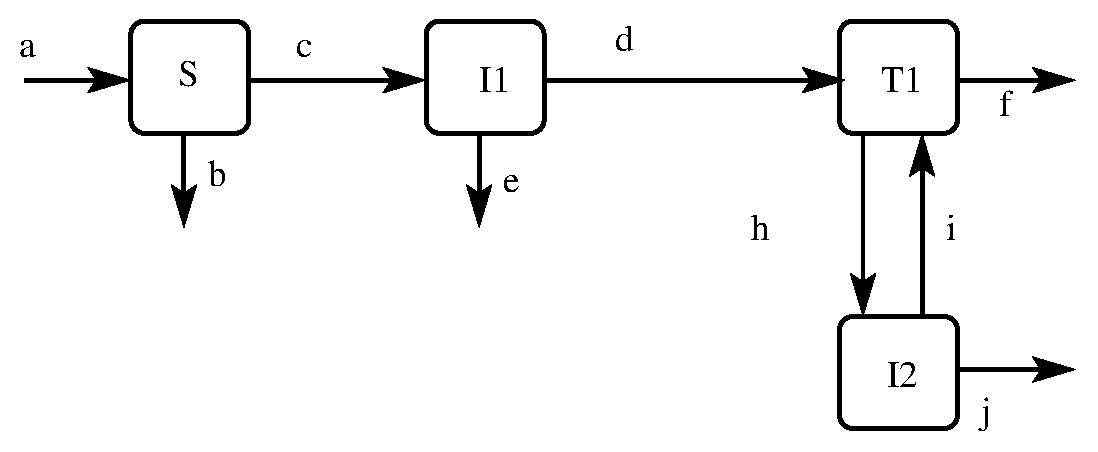
\includegraphics[width=14.5cm, height=5.5cm]{HIVModel_Dropout_ONLY.eps}
}
\end{center}
\caption{Model with dropout only. $\tau_i$, $\tau_T$ and $\tau_L$ are time since infection, time since treatment, and time since LTFU, respectively.}
\label{HIVmodel_SIT12}
\end{figure}

\begin{itemize}
 \item For class I, we would keep track of time since infection $\tau_i$.
 \item For class T, we would keep track of time on treatment $\tau_T$, time reset to zero.
 \item For class L, we would keep track of $\tau_L$, also here time resets.
\end{itemize}

We assume that death rate depends on:

\begin{itemize}
 \item time since infection for class I.
 \item only natural death for class T.
 \item time since LTFU for class L. 
\end{itemize}

We assume that transmission potential depends on:

\begin{itemize}
 \item time since infection for class I.
 \item for class T - does not depend on time since treatment. We consider average transmission probability of individuals who are not ART and then multiply that by a coefficient for the reduction effect due to HIV treatment. 
 \item time since LTFU for class L, but multiplied by a scaling parameter to account for a behavior change which we might see. If we assume the scaling parameter as 1 (equal infectiousness level), then it means an individual in L class who has been one year since LTFU is as infectious as an individual in I class who has been infected for one year.
\end{itemize}
 
 ART initiation depends on:
 \begin{itemize}
  \item time since infection, calendar time and ART access rate for class I.
  \item time since LTFU, calendar time and ART access rate for class L.
 \end{itemize}

 The rate of LTFU depends on time since treatment. \\ 
 
 Issues or decisions we might face:
 \begin{itemize}
  \item rate of ART re-initiation for class L.
  \item relative infectiousness level of class L as compared to I. Or just the infection rate due to class L.
  \item parameterization of dropout rate as a function of time since treatment.
  \item parameterization of HIV/AIDS induced death rate for classes T and L.
 \end{itemize}

 Note: If we assume that treated individuals are forced to stay on HIV treatment (no second-line) or dropout from ART, we won't have delays from implicit treatment failure. Losing the history of infection and treatment for class L is a limitation, but difficult to track both. 

 \end{document}
